\chapter{Leaf Identification}

\section{Introduction}
In this chapter we discuss the mechanics of leaf classification exploring two different approaches and evaluating the success or otherwise of both.

For this stage of the project it is more productive to develop the vision software using Java SE on the desktop instead of in the Android environment. As the same OpenCV library is being used both on the desktop and on Android it should make porting the techniques to another platform straightforward. This should offer an easier development path both in debugging and deployment as we remove the need to manage the extra complexity involved in deploying to a different platform. 


\section{Algorithmic Approach}

This approach revolves around extracting certain features from an image, such as edges, colour, textures, contours, etc. and creating a model to match that leaf type.

It is important to keep the number of transformations performed on the individual image minimal as this project is targeting a resource starved environment. The Android application will also be required to display a number of frames per second to provide a sense of real-time feedback to the user, although this may be achieved by processing only every second or third frame.

In this section we will concentrate primarily on identifying shapes, which removes the necessity to store and manipulate large sized images and colour information. 

The concept being tested in this section is to perform a series of transformations to differentiate the leaf from the background, this is hoped to enhance the leaf’s edges for a given frame and finally using contours to extract the shape of that leaf. 

\subsection{Resource Utilisation}

Early in the process we can combine the BGR (Blue, Green, Red) colour channels into a single grayscale channel and we may also sub-sample the image. These two optimisations will help minimise both CPU and memory utilisation.

Just to briefly describe the the gain from converting and storing the image in grayscale, we will analyse how the image is stored in OpenCV. The IplImage type that OpenCV operates on stores an image as a number of bitmaps, one for each channel of colour information. For this project we define that each pixel will have a colour depth of 256 shades per channel and this is stored in a 8bit unsigned structure, giving 1 byte per colour channel per pixel  \cite{morganIPL06}.

For example the video stream been analysed in the test environment has an resolution of 640 x 480 pixels which is 307,200 individual pixels. For each pixel we must record colour values for red, green and blue which require 1 byte each. To calculate the necessary memory we multiply 307,200 pixels by the 3 bytes which gives us 900 kilobytes per frame. If we are to convert the image to a single grayscale channel we save 600 kilobytes per frame. This equates to a considerable memory saving, especially when we see as many as 24 frames per second being processed.

The actual image size returned depends on the model of the device, for example the device being used for this project is the Google Nexus One which is capable of capturing 720 x 480 pixels at 20 frames per second.

This analysis is slightly simplistic as the IplImage type contains padding and metadata, but gives a good overview of the savings involved.

At this stage we are unable to provide an analysis of memory savings from sub-sampling performed on the image, as the optimal size for shape analysis is yet to be discovered.


\subsection{Preparing the Image}

\begin{figure}[h!]
\centering
    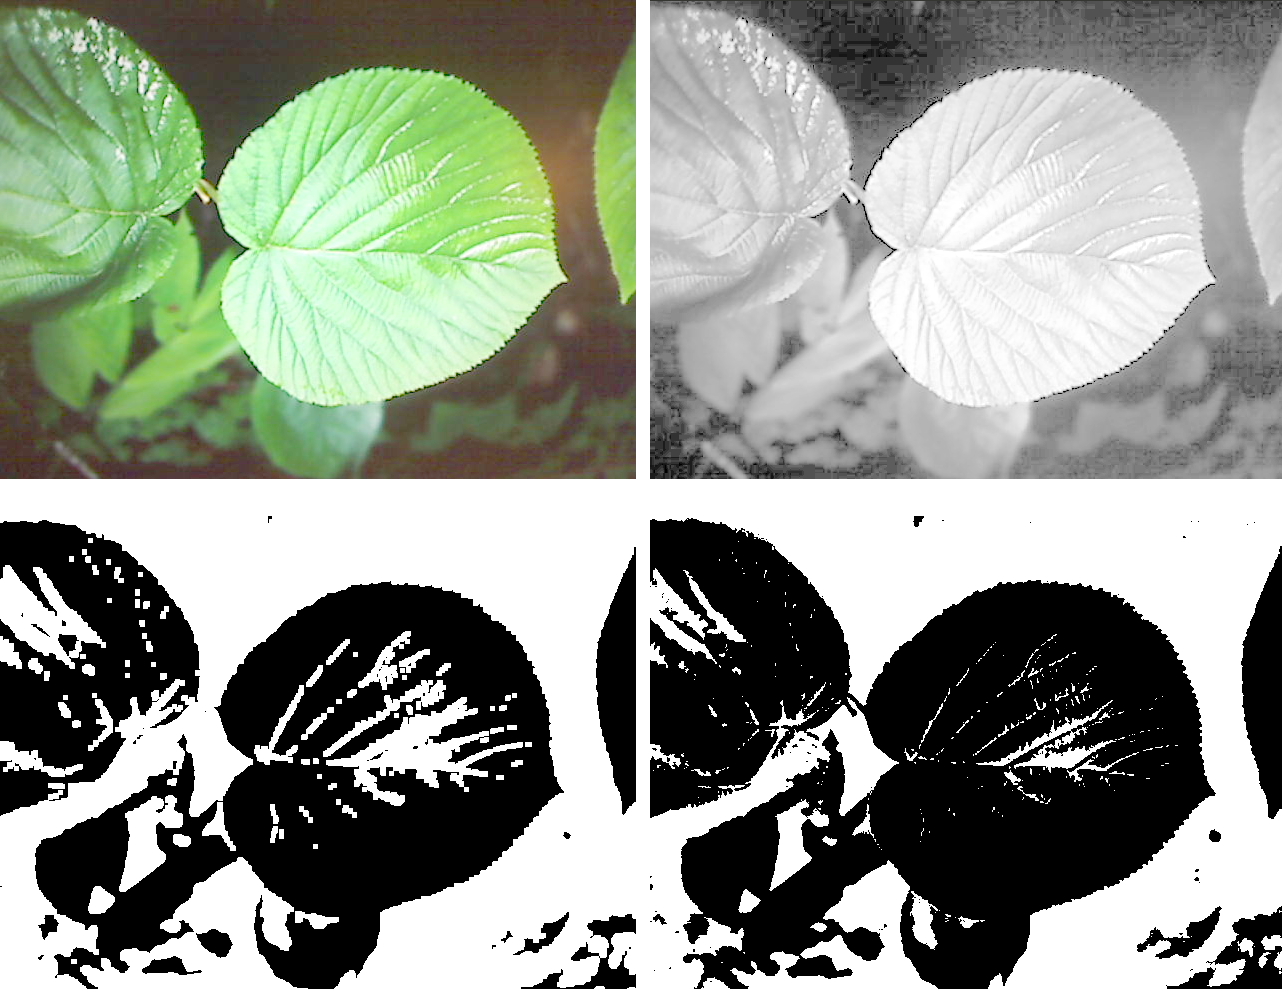
\includegraphics[width=1.0\textwidth]{leaf_identification/images/stages_of_processing.png}
    \caption{Stages of Processing: Input raw image (top left), Grayscale image with histogram equalisation (top right), Binary image after adaptive threshold (bottom right), Dilated binary image (bottom left)}%
    \label{stages_of_processing}
\end{figure}

Once a frame is retrieved from the camera's sensor we must preprocess the image before attempting to classify its features. The goal of preparing the image is twofold, firstly we need to perform filtering on the image in order to separate the foreground objects from the background, and secondly the \emph{cvFindContours()} function requires a binary image as input.

In Figure \ref{stages_of_processing} we can see a visual representation of the transforms performed on the image. The order and configuration of these have been determined through experimentation until a reasonable result was achieved. Below we describe the transformations and the order in which they are utilised.


\subsubsection{Convert to grayscale}
As discussed earlier we attempt to optimise any processing by minimising both the memory and CPU utilisation. As colour information is unnecessary for this approach we remove it at the first available opportunity.

It would be also advisable at this stage to sub-sample the image to the smallest size possible while still achieving good matches.

\subsubsection{Histogram Equalisation}
The image quality from mobile phone sensors vary widely, but one common problem that would hinder the classification of shapes in an image is the lack of contrast. With histogram equalisation we redistribute brightness across the range of the image, expanding the dynamic range of the image which increases the contrast \cite{kuntz09}.


\subsubsection{Binary conversion}
To detect contours we must first convert an image into its binary representation. There are a number of ways to perform such a conversion, with threshold and edge detection being most common.

In Figure \ref{preprocessing} we see the results of processing an image with the Canny Edge detection (left) and the Adaptive Threshold (right) algorithms. On inspection of the output it is clear that the adaptive threshold function provides a better silhouette of the central object, edge detection gives a broken ‘contour’ of the leaf. 

To evaluate which technique offers the best result, we must understand what a contour is and how they are detected. We will discuss this further later in the document but for our purposes here a contour is a curve drawn on the boundary between light and dark areas of a binary image, these are typically closed and may contain further nested curves.

With this in mind we see in Figure \ref{preprocessing} that the adaptive threshold approach offers a clearer representation of the shape. At this point it might be important to point out that it may be useful to utilise edge detection to enhance the edges of an image before conversion to its binary form. This may help to add further definition to the foreground object.

When applying a threshold filter to an image we are essentially making a decision to accept or reject a particular pixel based on a certain threshold value \cite{bradski08}. OpenCV provides a number of options for how the threshold is to be calculated.

Adaptive threshold is a technique where the threshold value is variable, this threshold value is calculated as a weighted average from a predetermined pixel region around the current pixel.

Once this transform is applied to the input image we are returned a binary version of that image which can then be used to find contours, we will discuss this further in the next section.

\begin{figure}[h!]
\centering
    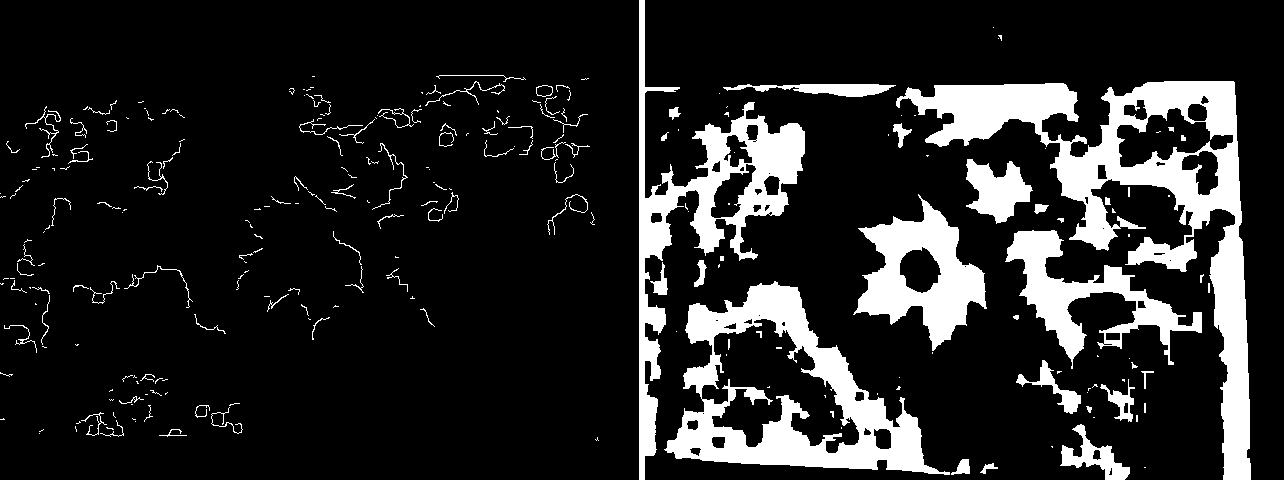
\includegraphics[width=1.0\textwidth]{leaf_identification/images/convert_to_binary.png}
    \caption{Binary image conversion: Canny Edge detection (left) and Adaptive Threshold (right)}%
    \label{preprocessing}
\end{figure}


\subsubsection{Dilate}
After an image has been converted to its binary representation, we must to attempt to eliminate noise which may have crept in from the previous processing steps. Noise concentrated on a boundary in an image may adversely affect the contours that are extracted. 

Due to the nature of the images we are processing, it is important to perform minimal noise reduction. If we were to over correct for noise we would inadvertently affect the shape of the detected object, decreasing the systems accuracy.

Typically erosion and dilation transforms are applied to an image in order to decrease or remove noise \cite{bradski08}. Dilation has the effect of making bright regions in an image glow or expand, while erosion has the opposite effect. These functions use a pixel mask with an anchor point to scan the input image and calculate the local maximum value in the case of dilate or local minimum value in the case of erode. As this mask is then passed over the image, the anchor point pixel value is set to that of the local maximum or minimum for this mask.

As stated previously we aim to preform only minimal noise correction, it was decided to apply a dilate transform with a small mask size. Dilation was decided upon as the type of images being processed my have very thin borders and this technique is the best for preserving these edges.




\subsubsection{Additional techniques}
We are battling a number of constraints in this environment namely lighting conditions, shade variation between background and foreground items, non-uniformity in the shape of the leaves as well as designing performant software. After experimenting with a number of different techniques for creating a good binary representation the procedure outlined above was settled on.

However, a number of enhancements could be made to the process with the aim of increasing accuracy. 

\begin{itemize}
\item Enhance the edges of the preprocessed image using edge detection
\item Alternate the type of preprocessing performed on each frame
\item Background subtraction
\item Dynamic preprocessing using use values from the last captured image such as average brightness and shade range between average brightness and darkness to process the image based on its actual conditions
\end{itemize}


\subsection{Identifying features}

As seen in Figure \ref{preprocessing}, we should now have a clean binary image with the object of interest being identifiable to the eye. We must now use some mechanism to detect shapes and compare them to a store of pre-captured shapes in an efficient manner. 


\begin{figure}[h!]
\centering
    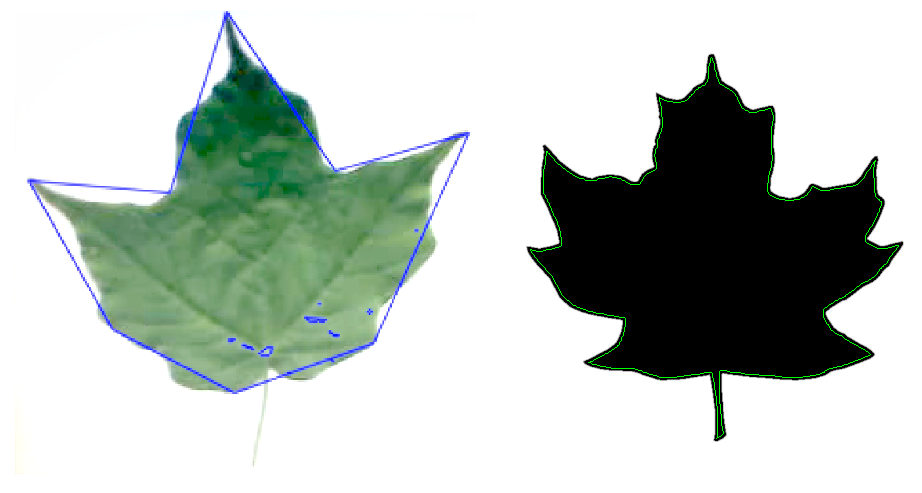
\includegraphics[width=1\textwidth]{leaf_identification/images/contours.png}
    \caption{Contour detection: Early crude detection (left), Extracting an accurate reference contour for a leaf (right)}%
    \label{contours}
\end{figure}

\subsubsection{Contours}

OpenCV provides the function \emph{cvFindContours()} which maps boundaries in a binary image. A contour is essentially a list of points that represent a curve in an image \cite{bradski08}. While obvious, it is important to point out that the contours returned are the result of the image preprocessing and may not represent the actual items being captured.

The function returns a contour tree, which is a nested structure of all the contours discovered. This concept of contours containing further contours is useful for certain forms of shape analysis. A individual contour is returned as a sequence of \emph{(x,y)} points that describe the edge of an object. In Figure \ref{contours} the reference contour (left) is composed of a sequence of some 699 points, we consider this the raw contour.


\subsubsection{Polygon Approximations}
In the returned nested structure of raw contours we have a contour that matches the binary shape of interest. We need to generalise the shape of the contour to create a more generic representation of the shape. This will help to correct for defects in the image and the physical leaf, to remove artifacts from the processing and to minimise the number of points in the contour sequence for storage. 

We apply the \emph{cvApproxPoly()} polygon approximation function which attempts to approximate the contour with that of one containing fewer vertices's. OpenCV provides an implementation of the Ramer-Douglas-Peucker approximation algorithm which we use to perform this approximation. This function takes the contour and a precision value as an input. The precision value defines the minimum distance points must be apart before inclusion in the new contour.

The algorithm begins by joining the two points in the polygon with the greatest distance between them, then recursively joins all the points until the precision value is encountered \cite{ramer72, bradski08}.

Once we apply this approximation function to our raw contour in Figure \ref{contours_raw_approx} we reduce the number of points from 699 to 126 while retaining the shape of the object.

\begin{figure}[h!]
\centering
    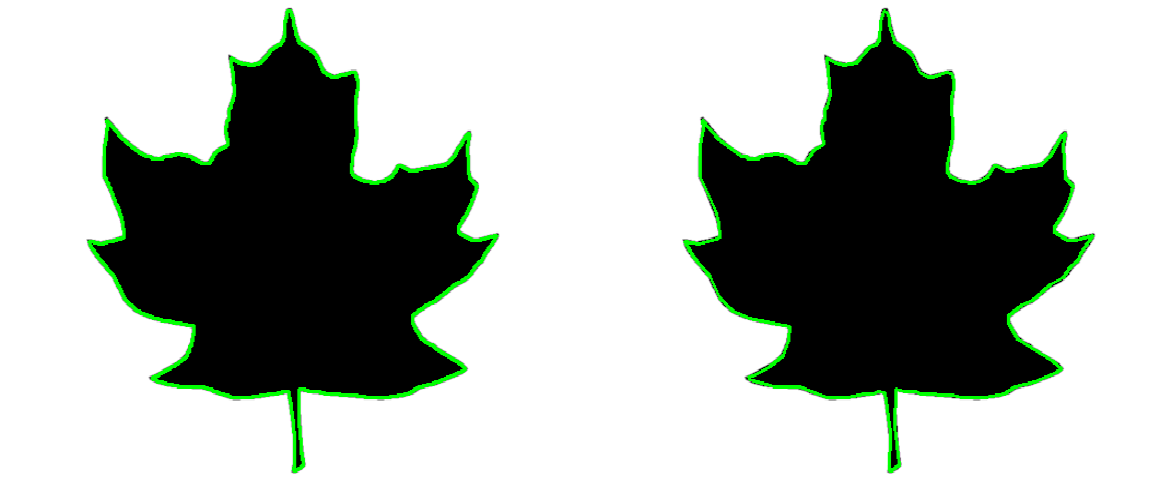
\includegraphics[width=1\textwidth]{leaf_identification/images/contours_raw_approx.png}
    \caption{Polygon Approximation: Raw contour (left) containing 699 points, Contour approximation (right) containing 126 points}%
    \label{contours_raw_approx}
\end{figure}

\subsubsection{Shape Matching}
Now that we have accurate contours from the object being captured by the camera and a collection of reference contours from known leaf types we must compare these shapes to categorise the object.

Again OpenCV provides mechanisms to perform this comparison, they are contained in the function \emph{cvMatchShapes()}. This function takes two contours and a value to select the comparison metric as its input, and returns a numeric value which describes how similar the shapes are with 0 being a match. This comparison is made using Hu invariant moments, which we will describe below.

From exposing many different silhouettes of leaves it was determined that a value of less than 0.03 can be considered to be a good match. However it is likely that with a larger database of leaf types to compare a more precise match may be required.

An image moment defines a gross characteristic of a contour which is calculated from the integral of all the pixels in the contour. These moment’s can be used to compare two contours, but will only match contours of the same shape, size and rotation.

Hu invariant moments provide the ability to match shapes under translation, so changes in their scale, rotation or reflection will not effect a match being made \cite{shutler02, rizon06}.

\colorbox{red}{would be nice to expand on hu moments}

\subsubsection{Additional techniques}
Using Hu invariant moments to compare two shapes has proven to be quite accurate. While other options such as chain codes such as Freeman’s offer an interesting alternative \cite{park05}. Histogram to detect shapes under rotation Figure \ref{chain_codes}


In addition to chain codes, calculating convexity defects from a convex hull of the shape \cite{iivarinen97}. 

\begin{figure}[h!]
\centering
    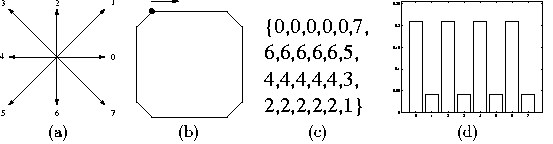
\includegraphics[width=.7\textwidth]{leaf_identification/images/chain_codes.png}
    \caption{Chain codes}%
    \label{chain_codes}
\end{figure}

\subsection{Storage and Retrieval}
To describe a leaf before applying polygon approximations we see in the region of 700 Cartesian points, \colorbox{red}{how may after??}. Efficient lookup and storage of these leaf signatures is going to prove to be a difficult task.

For this project the approach used was to load a flat file of contours into memory, storing this form of data in a relational structure would be massively inefficient.

It is clear that as the size of the library increases a lookup mechanism would be required, removing the need to store all contours in memory.


%%%%%%%%%%%%%%%%%%%%%%%%%%%%%%%%%%%%%%%%%%%%%%%%%%%%%%%%%%%%%%%%%%

\section{Machine Learning Approach}
haarcascade classifier

\colorbox{red}{How to partiton the set in multiple ways - as paddys suggestion}

\subsection{Training Set}

\subsubsection{Positive Images}
between 2500 - 5000 images recommended
different lighting, angles etc

\subsubsection{Negative Images}
3000 negative image - do not contain object in question

\subsubsection{Natural Test Images}

\subsubsection{Preparing the dataset}
Use http://code.google.com/p/imageclipper/ 
All images must have the same size
